\chapter{重整化、自然性與層級問題}

\lectureoverview{本課程的核心思想源自標準模型中關於重整化的種種疑問。因此，我們先從重整化的物理意義談起：消去對當前問題而言過小、變化過快的自由度，再將其效應納入有效描述。分子提供了一個典型範例。接著，量綱分析把相同的推理帶入標量量子場論，揭示標量質量對截斷尺度的二次敏感性、希格斯場的層級問題、費米子與規範玻色子所受到的保護，以及更嚴重的真空能問題。}

\section{依問題尺度而定的物理}

本季將探討的大部分思想，都源自標準模型中關於重整化的問題---有時是疑難，有時是有用的觀察---。重整化結合了兩種思考方式。第一種是從描述中移除距離短到與當前問題無關的結構。第二種是量綱分析；它往往能在計算任何困難的積分之前，就決定短距離下的答案。

這種剔除細節的做法遍及物理學各領域。若要理解原子核，可以從夸克和量子色動力學出發。算出質子與中子的質量、自旋，以及它們所產生的有效核力之後，在許多情況下就可以不再理會它們的夸克次結構。核的運動足夠緩慢，因此以質子和中子為對象的非相對論量子力學，往往是更有用的描述。

到了下一個層次，原子物理通常不必理會原子核的內部組成。核物理告訴我們有哪些原子核和同位素，也提供質量、電荷等性質。於是我們以一組新的有效基本物件重新開始：原子核和電子。夸克、質子和中子並未消失；它們的效應已濃縮在原子核所帶有的參數之中。

要保留多少資訊，取決於接下來要回答什麼問題。原子計算可能需要核質量，因為它會進入約化質量；當然也需要核電荷，因為它決定庫侖場。通常不必知道各夸克分別攜帶多少核動量。元素的核電荷約有九十種，若計入同位素，核種還會更多。這份目錄可以直接作為輸入。另一方面，電子還不能消去：原子結構正是由電子的運動形成的。

解出原子問題後，我們也可以把原子視為分子的構建單元。Susskind 列出的曲奇原子、咖啡原子、巧克力原子和番茄醬原子，雖然異想天開，卻點出了嚴肅的道理：每個層次都有新的描述。一旦知道分子的性質和作用力，就能把分子組合成更大的 Tinkertoy 式結構，不必每一步都重新處理電子問題。

每一次這樣的轉換都是一次粗粒化。新的描述在絕對意義上或許不那麼精確，但在預定的尺度上實用得多。量子場論無法避開這個問題，因為場在每個波長上都有模式，波長甚至可以任意短。因此，我們把短到無法解析的波長所產生的效應加總，再以新的有效參數取代這些細節。這項操作連同量綱分析，構成了重整化的物理內涵。

\section{分子：典型範例}

考慮兩個原子，並試著簡單描述它們的相對運動。每個原子都由一個重原子核和一團電子雲組成。即使是質子，質量也約為電子的兩千倍；更重的原子核則讓兩種尺度相差更大。一個有用的圖像是：兩顆保齡球周圍有一群快速飛舞的蒼蠅——原子核反應緩慢，電子態則迅速重新排列。

令原子核的位置和動量分別為 \(R_a\) 和 \(P_a\)，共同質量為 \(M\)；電子的座標和動量分別為 \(r_i\) 和 \(q_i\)，質量為 \(m_e\)。略去 \(4\pi\epsilon_0\) 等慣用因子後，哈密頓量的示意形式如下：
\begin{align}
H={}&
\frac{P_1^2}{2M}+\frac{P_2^2}{2M}
+\frac{e^2}{R_{12}}
+\sum_i\frac{q_i^2}{2m_e}
+\frac12\sum_{i\ne j}\frac{e^2}{r_{ij}}
\nonumber\\
&-\sum_i\left(
\frac{e^2}{|R_1-r_i|}
+\frac{e^2}{|R_2-r_i|}
\right).
\label{eq:molecular-hamiltonian}
\end{align}
第一行包括原子核的動能、原子核彼此之間的庫侖排斥，以及電子的動能。第二行包括電子彼此之間的排斥和電子與原子核之間的吸引。若原子核的電荷一般記為 \(Z_a\)，就要補回相應因子；本講將電荷寫成示意形式，是因為重點在於時間尺度的分離。

這裡有兩種特徵運動：原子核質量大、運動慢；電子質量小、運動快，快到看起來像一團模糊的影像。第一步近似是固定原子核的位置，並將所有依賴電子座標的項合併成電子哈密頓量：
\begin{equation}
H_{\mathrm{el}}(R_1,R_2).
\end{equation}
對每一種固定的原子核構型，求解
\begin{equation}
H_{\mathrm{el}}(R_1,R_2)
\psi_0(r_1,\ldots,r_N;R_1,R_2)
=
E_{\mathrm{el}}(R_1,R_2)\psi_0.
\label{eq:electronic-ground-state}
\end{equation}
我們保留最低的電子本徵值。電子並未被忽略；它們所有快速運動的效應，都已由函數 \(E_{\mathrm{el}}(R_1,R_2)\) 概括。

這套推理採用絕熱近似。在電子快速調整的一段時間內，原子核移動極少，因此可以把它們的座標視為參數。解出電子本徵值問題後，再讓同一組座標恢復運動。每當構型緩慢改變，電子雲便跟隨當下的基態。更精確的處理可以納入激發的電子態勢能面，以及不同態之間的躍遷；不過，最低能態勢能面已足以呈現重整化的概念。

\begin{figure}[htbp]
\centering
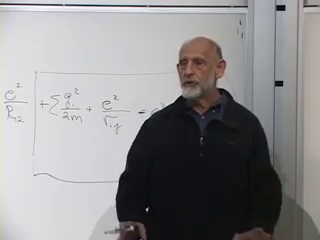
\includegraphics[width=0.72\textwidth]{lecture_01_figure_02.png}
\caption{介紹電子基態問題時，分子哈密頓量仍留在黑板上。式~\eqref{eq:molecular-hamiltonian}的排版形式列出了畫面中被遮住的各項。}
\lectureframe{00:16:19}
\end{figure}

\begin{classroomqa}
\audiencequestion{原子核的動量只是被設為零嗎？\lecturetimestamp{00:15:39}}
\lecturerresponse{只是暫時如此。在最低階近似中，原子核被視為固定不動，因為它們的運動遠比電子慢。求解有效的原子核問題時，我們會把原子核的動量納入，因此這項近似並未違反不確定性原理。}
\end{classroomqa}

電子基態能量現在成為原子核所感受到的有效位能的一部分：
\begin{equation}
V_{\mathrm{eff}}(R_1,R_2)
=\frac{e^2}{R_{12}}+E_{\mathrm{el}}(R_1,R_2).
\label{eq:molecular-effective-potential}
\end{equation}
對兩個孤立原子而言，轉動和平移不變性使這個位能只依賴兩原子間距 \(R_{12}\)。在距離極短時，原子核之間的庫侖排斥占主導；距離極遠時，交互作用很弱。在這兩個極限之間，電子雲可以形成吸引區域和一個極小值。原子核的波函數因而集中在該極小值附近，描述出一個束縛分子。

請注意運算順序。我們並不是猜出一個經驗上的吸引力就把電子丟開，而是先在固定的原子核背景下求解電子的量子問題，之後才消去電子的顯式座標，保留所得的本徵值。短距離物理的效應保留在 \(V_{\mathrm{eff}}\) 的形狀、深度和曲率之中。極小值的位置決定平衡間距；曲率決定小振動的性質；漸近形式則決定束縛態是否存在。一個有效函數就把所有這些電子資訊帶入較慢的問題。

因此，複雜的多電子哈密頓量已轉化為帶有新位能的雙原子核哈密頓量。我們消去了快速自由度，同時完整保留它們對低能物理的影響。這個位能經過了重整化。熟悉的 Born--Oppenheimer 推理通常不以重整化之名介紹，卻恰好包含我們需要的概念：
\begin{equation}
\begin{gathered}
\text{fast microscopic dynamics}\\
\Downarrow\\
\text{effective parameters for slow dynamics}
\end{gathered}
\end{equation}

\section{自然單位制與場的量綱}

在量子場論中，要消去的模式也可以稱為短距離、短波長、高頻率或高能量模式。在畫費曼圖之前，先確定量綱的計算方式。

一般力學使用彼此獨立的長度、時間和質量單位。在粒子物理中，我們令
\begin{equation}
\hbar=c=1.
\end{equation}
如此一來，能量和質量由 \(E=mc^2\) 聯繫起來；由於 \(c=1\)，長度和時間等價；而 \(\hbar=1\) 使動量成為長度的倒數。最後只剩下一種量綱：
\begin{equation}
[M]=[E]=[p]=L^{-1},
\qquad
[x]=[t]=L.
\label{eq:natural-units}
\end{equation}

這並沒有消除量綱，而是選定換算因子，讓時間可以用長度表示，質量可以用長度的倒數表示。只要指定一個單位，其他單位就都隨之確定。因此，截斷尺度既可以用短距離 \(\delta\) 描述，也可以用高能量 \(\Lambda=1/\delta\) 描述：兩者只是同一尺度的不同說法。

考慮一個實標量場 \(\phi\)，其拉格朗日密度採用以下示意性的正規化：
\begin{equation}
\mathcal L=(\partial_\mu\phi)(\partial^\mu\phi)-V(\phi),
\qquad
S=\int d^4x\,\mathcal L.
\label{eq:scalar-action}
\end{equation}

\begin{figure}[htbp]
\centering
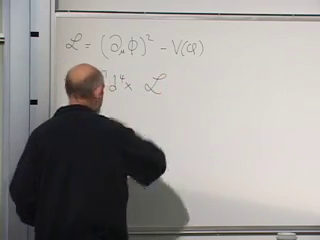
\includegraphics[width=0.78\textwidth]{lecture_01_figure_03.png}
\caption{局域的標量拉格朗日密度，以及將它對時空積分所得的作用量。}
\lectureframe{00:26:08}
\end{figure}

拉格朗日密度是局域的，描述單一時空點。經典場方程由作用量取駐值的條件導出。在量子理論中，同一個作用量出現在路徑積分的相位 \(\exp(iS)\) 中。無論採用哪種觀點，\(S\) 的量綱都至關重要。恢復 \(\hbar\) 後，相位為 \(\exp(iS/\hbar)\)；令 \(\hbar=1\) 後，\(S\) 本身必須是無量綱的。

\begin{classroomqa}
\audiencequestion{作用量的單位是\(\hbar\)嗎？\lecturetimestamp{00:26:13}}
\lecturerresponse{是的。既然 \(\hbar\) 已設為一，作用量在這套單位制中就是無量綱的。四維積分測度的量綱是 \(L^4\)，因此拉格朗日密度的量綱必須是 \(L^{-4}\)。}
\end{classroomqa}

現在由動能項決定場的量綱：
\begin{align}
[S]&=1, & [\mathcal L]&=L^{-4},\\
[\partial_\mu]&=L^{-1}, &
[(\partial\phi)^2]&=L^{-2}[\phi]^2=L^{-4},\nonumber\\
&& [\phi]&=L^{-1}.
\label{eq:scalar-dimension}
\end{align}
這個簡單的計算將決定後續所有圖在紫外區的量綱。

將位能展開為
\begin{equation}
V(\phi)=\frac{m^2}{2}\phi^2+g\phi^3+\lambda\phi^4+\cdots.
\label{eq:scalar-potential}
\end{equation}
每一項的量綱都必須是 \(L^{-4}\)。由於
\([\phi^n]=L^{-n}\)，
\begin{equation}
[m^2]=L^{-2},
\qquad
[g]=L^{-1},
\qquad
[\lambda]=1.
\label{eq:coupling-dimensions}
\end{equation}
四次耦合是無量綱的。這類耦合在重整化中特別重要，因為它們對尺度的依賴性無法單從長度的簡單冪次看出。

\begin{classroomqa}
\audiencequestion{\(g\)的單位是質量嗎？\lecturetimestamp{00:29:52}}
\lecturerresponse{是的。因子 \(\phi^3\) 的量綱是 \(L^{-3}\)，而位能密度的量綱必須是 \(L^{-4}\)。因此 \([g]=L^{-1}\)；在自然單位制中，它的量綱就是質量。}
\end{classroomqa}

\section{頂點與短距離傳播子}

費曼規則由頂點和傳播子構成。\(g\phi^3\)項提供一個三線頂點，其因子正比於 \(g\)；\(\lambda\phi^4\)項提供一個四線頂點，其因子正比於 \(\lambda\)。二次項則提供一個局域的兩點插入。可以把它想成一個粒子進入後被吸收，再重新發射出來；其係數正比於 \(m^2/2\)。本講刻意略去數值正規化、正負號、\(i\) 的因子和對稱因子，因為重點在於找出尺度依賴性，而非計算散射截面。

這些圖有其操作上的詮釋。三點頂點可以吸收兩個量子並發射一個量子，也可以代表三條線的其他交叉相關配置。四點頂點可以描述兩個粒子入射、兩個粒子出射。二次項的交叉符號仍代表合法的兩線頂點，雖然通常會把它併入自由傳播子中。我們把它畫出來，是因為稍後可以藉由比較，辨認出每一種未解析的兩點過程。

傳播子連結兩個時空點。圖中的線並不表示量子粒子沿著經典直線運動，而是代表在 \(x\) 產生場激發，並在 \(y\) 將它移除或探測到的振幅：
\begin{equation}
\Delta(x-y)=\langle0|\phi(y)\phi(x)|0\rangle.
\label{eq:position-propagator}
\end{equation}
從右向左讀這個式子。\(\phi(x)\)作用在真空上，會在 \(x\) 產生一個單粒子成分。\(\phi(y)\)作用在左矢上，則移除 \(y\) 的成分。它們的真空矩陣元是第一個時空點產生粒子、第二個時空點探測粒子的重疊振幅。符號 \(x\) 和 \(y\) 代表完整的四向量，不只是兩個笛卡兒座標。

態不帶物理量綱，而每個場帶有量綱 \(L^{-1}\)。因此
\begin{equation}
[\Delta]=L^{-2}.
\end{equation}
無質量場沒有內在的長度尺度，所以量綱分析決定其短距離行為為
\begin{equation}
\Delta(x-y)\sim\frac{1}{(x-y)^2}.
\label{eq:massless-propagator}
\end{equation}
分母是洛侖茲不變的間隔平方；在奇點處須採用通常的處方。\editorialnote{為了進行冪次計數，將間隔作 Wick 轉動至歐幾里得時空會更方便；此時其大小明確地正比於 \(1/|x-y|^2\)。這不會改變以下分析所用的紫外冪次。}

當 \(y\) 趨近 \(x\) 時，傳播子會發散。這種間隔趨近於零時的傳播奇異性，正是更複雜圖形中紫外發散的來源。

\section{標量質量的重整化}

對標量場而言，動力學參數是 \(m^2\)，這點已可從相對論性的色散關係看出：
\begin{equation}
E=\sqrt{\mathbf p^2+m^2}.
\end{equation}
令 \(\delta\) 為有效描述所能解析的最短距離。若頂點間距小於 \(\delta\)，我們便不加以區分。任何這類未解析過程，只要有一個入射標量和一個出射標量，其可觀測的兩點結構就與質量插入相同，因此必須對有效質量有所貢獻。

可以把加速器想成顯微鏡。若它最精細的解析度是 \(\delta\)，那麼在一處吸收、又在遠小於 \(\delta\) 的距離外發射，便無法和真正的局域事件區分。我們刻意在這個尺度上模糊頂點。重整化的規則，就是把所有這類低於解析度、彼此無法區分的過程，納入相應局域算符的係數。

\subsection{第一個四次作用修正}

從一個 \(\phi^4\) 頂點開始。兩條線是外部粒子；另外兩條線形成短迴圈，在幾乎同一點發射並重新吸收。把重合點的傳播子在截斷距離上平滑化，可得
\begin{equation}
\Delta(0)\ \longrightarrow\ \Delta(\delta)\sim\frac{1}{\delta^2},
\end{equation}
因此
\begin{equation}
\delta m^2_{(1)}\sim\frac{\lambda}{\delta^2}.
\label{eq:one-loop-scalar-mass}
\end{equation}
若 \(m_0^2\) 表示輸入參數，也就是裸參數，則低解析度下的兩點係數示意為
\begin{equation}
\frac{m_{\mathrm{eff}}^2}{2}
\sim
\frac{m_0^2}{2}
+c_1\frac{\lambda}{\delta^2},
\label{eq:first-renormalized-mass}
\end{equation}
其中 \(c_1\) 包含此處略去的數值因子和依賴慣例的因子。在無法解析小於 \(\delta\) 距離的實驗中，所測得的實驗室質量就是這個重整化後的量，而非單獨的 \(m_0\)。

因此，觀測到的兩點事件有兩種無法區分的發生方式：原有的二次頂點吸收並重新發射粒子，或者四次交互作用在短暫發射並重新吸收一個虛標量粒子的同時，造成相同結果。量子力學會將振幅相加。當迴圈的尺度低於解析度時，它獨立的歷程不再出現在有效描述中，但它對測得係數的貢獻仍然存在。

\subsection{下一個四次作用修正}

現在把兩個四次頂點連接起來：一個外部粒子從 \(x\) 入射，另一個從 \(x+\Delta\) 出射，兩個頂點之間由三個內部傳播子連接。這裡有兩個 \(\lambda\) 因子，而傳播子則給出 \(\Delta^{-6}\)。量子振幅必須對所有無法解析的出射位置加總，因此要對相對四向量積分：
\begin{equation}
\delta m^2_{(2)}
\sim
\lambda^2
\int_{|\Delta|\gtrsim\delta}
d^4\Delta\,\frac{1}{|\Delta|^6}.
\label{eq:two-loop-power-count}
\end{equation}

\begin{classroomqa}
\audiencequestion{頂點旁的小標記表示那裡只有三個粒子嗎？\lecturetimestamp{00:46:35}}
\lecturerresponse{不是。我們用的仍是四次交互作用，每個頂點都有四條線相接。在這個兩點圖中，一條是外線，另外三條在兩個頂點之間延伸。第二個頂點也同樣有四條線相接。}
\end{classroomqa}

積分測度貢獻長度的四次方，而三個傳播子合計貢獻長度的負六次方。由於紫外截斷是估算中唯一的尺度，
\begin{equation}
\int_{|\Delta|\gtrsim\delta}
\frac{d^4\Delta}{|\Delta|^6}
\sim\frac{1}{\delta^2},
\qquad
\delta m^2_{(2)}
\sim\frac{\lambda^2}{\delta^2}.
\label{eq:two-loop-scalar-mass}
\end{equation}
這裡的 \(\Delta^\mu\) 是四分量積分變數；積分涵蓋時間分量和三個空間分量。小寫的 \(\delta\) 則是固定的截斷距離。講課時一開始對兩者使用相同的口頭稱呼，之後才更正記號。

把四維測度改寫成徑向形式，也能看出相同結果。略去角度積分所給的常數，
\begin{equation}
\int_{\delta}\frac{d^4\Delta}{|\Delta|^6}
\sim
\int_{\delta}\frac{R^3\,dR}{R^6}
=\int_{\delta}\frac{dR}{R^3}
\sim\frac{1}{\delta^2}.
\end{equation}
因此，大距離端的積分上限對紫外估算並不重要：積分主要由下限決定。

更高階的圖也遵循相同模式。包含更多四次頂點的圖會帶來更高次的 \(\lambda\)，但量綱分析仍允許質量修正呈二次發散：
\begin{equation}
\begin{aligned}
m_{\mathrm{eff}}^2
={}&m_0^2
+\frac{1}{\delta^2}
\left(c_1\lambda+c_2\lambda^2+c_3\lambda^3+\cdots\right)\\
&+\text{weaker terms}.
\end{aligned}
\label{eq:scalar-mass-series}
\end{equation}

\subsection{三次交互作用與對數發散}

兩個三次頂點之間有兩個傳播子，連接鄰近的時空點。其貢獻的尺度關係為
\begin{equation}
\delta m_g^2
\sim
g^2\int_{|\Delta|\gtrsim\delta}
\frac{d^4\Delta}{|\Delta|^4}.
\label{eq:cubic-loop}
\end{equation}
此時測度和分母帶有相同的冪次，因此剩下的是對數依賴，而非冪次依賴：
\begin{equation}
\delta m_g^2
\sim
c_g g^2\log\!\left(\frac{1}{\mu\delta}\right).
\label{eq:cubic-log}
\end{equation}
參考尺度 \(\mu\) 使對數的引數成為無量綱量。這就是講課中示意寫法 \(g^2\log\delta\) 的完整量綱形式。對數的變化遠比任何逆冪緩慢，因此截斷距離縮短時，\(1/\delta^2\) 會占主導。

徑向形式再次清楚呈現這項差異：
\begin{equation}
\int_{\delta}^{R_{\mathrm{IR}}}
\frac{d^4\Delta}{|\Delta|^4}
\sim
\int_{\delta}^{R_{\mathrm{IR}}}\frac{R^3\,dR}{R^4}
=\log\!\left(\frac{R_{\mathrm{IR}}}{\delta}\right).
\end{equation}
測度和分母的冪次相同時會產生對數；分母的冪次較高時，則產生截斷距離的逆冪。這裡不需要計算角度因子；講課的目的，是教我們一眼看出紫外行為。

\begin{classroomqa}
\audiencequestion{這裡的對數是以什麼為底？\lecturetimestamp{00:57:42}}
\lecturerresponse{使用自然對數。改變底數只會乘上一個數值常數，而這個常數會併入係數中。此處尚未計算該係數內的 \(2\)、\(\pi\) 和對稱因子。}
\end{classroomqa}

\begin{classroomqa}
\audiencequestion{對長度取對數，量綱上不會出問題嗎？質量修正的量綱又從何而來？\lecturetimestamp{00:58:32}}
\lecturerresponse{對數比較的總是兩個尺度；嚴格來說，取對數的必須是 \(1/(\mu\delta)\) 這類無量綱比值。耦合 \(g\) 的量綱是質量的一次方，因此 \(g^2\) 的量綱恰好是質量平方，符合修正項所需的量綱。}
\end{classroomqa}

\begin{classroomqa}
\audiencequestion{費曼圖給出振幅。振幅的絕對值平方就是機率嗎？\lecturetimestamp{00:59:41}}
\lecturerresponse{若把振幅放進實際的躍遷計算，並納入所需的態因子和相空間因子，是的。這裡更直接的用途則不同：未解析的兩點振幅具有與質量項相同的局域形式，因此會改變有效質量參數。}
\end{classroomqa}

\section{所有參數都會成為有效參數}

質量修正圖形有無窮多個，並不會因為 \(\lambda\) 很小就消失。微擾論依耦合常數的冪次排列這些圖，因此後續各項可能逐次變小，但圖形仍有無窮多個。同樣的短距離消去也會使交互作用本身受到重整化。

\begin{classroomqa}
\audiencequestion{即使是質量重整化，也有無窮多個圖形嗎？\lecturetimestamp{01:00:35}}
\lecturerresponse{沒錯。如果 \(\lambda\) 足夠小，微擾級數可能仍然有用，因為高次項會逐次受到抑制。不過，重整化後的參數由整個級數定義，而不只由第一個圖形決定。}
\end{classroomqa}

從操作上來說，局域的 \(\lambda\phi^4\) 交互作用就是一個兩粒子入射、兩粒子出射的振幅。若更複雜的四點過程完全發生在無法解析的區域內，在低解析度下便無法和原來的局域頂點區分。因此，這些圖形都併入有效的 \(\lambda\)。在四維 \(\phi^4\) 理論中，它們的主導尺度依賴通常呈對數形式。本講並未計算該貝他函數，而是以此例說明一項普遍原則：
\begin{equation}
\begin{gathered}
\text{parameters measured at low energy}\\
\ne\\
\text{parameters entered at the microscopic cutoff}
\end{gathered}
\end{equation}

四點例子很重要，因為它排除了可能的誤解：重整化不是只用來處理質量發散的特殊修補。拉格朗日量中每個允許的算符，都可以由具有相同外部線和對稱性的未解析圖形再現。兩點過程會重整化二次項係數，四點過程會重整化四次項係數，而真空到真空的過程則會重整化常數項。低能拉格朗日量是一份精簡的帳目，記錄了所有這些短距離過程。

\begin{classroomqa}
\audiencequestion{既然 \(\Delta\) 的量綱是長度，對它取對數在量綱上不會有問題嗎？另外，黑板上的大寫和小寫 delta 是否曾經對調？\lecturetimestamp{01:01:34}}
\lecturerresponse{這裡的對數實際上是尺度之比，因此是無量綱的。沒錯，記號一度對調：\(\Delta^\mu\) 是積分變數，而 \(\delta\) 是最後留在答案中的最小距離截斷。}
\end{classroomqa}

這是分子範例在場論中的對應情況。我們解出不可見的快速電子所產生的效應，並將結果納入位能。此處則是加總不可見的短距離過程，再將結果納入質量、耦合常數和其他所有允許的局域係數中。所有參數都會改變。

\begin{classroomqa}
\audiencequestion{可以再說明一次嗎？測得的量是否包含實驗看不到的更小尺度所產生的效應？\lecturetimestamp{01:05:13}}
\lecturerresponse{是的。這些尺度上的個別漲落無法解析，但加總後的效應仍然存在。所有涉及更短尺度的圖形都會合併到單一有效係數中；低能實驗稱這個係數為物理質量平方等參數。}
\end{classroomqa}

\begin{classroomqa}
\audiencequestion{那輸入項 \(m_0^2\) 是否必須抵消其他貢獻？\lecturetimestamp{01:06:00}}
\lecturerresponse{如果測得的標量質量遠小於各個紫外貢獻，就必須如此。這種所需的抵消，就是接下來要談的精細調節問題。}
\end{classroomqa}

\section{希格斯層級問題}

假設截斷距離就是普朗克長度，那麼有效場論就得概括從實驗室尺度到量子重力必須介入之尺度間的漲落。
以粒子物理單位表示，
\begin{equation}
\delta\sim M_{\mathrm{Pl}}^{-1}\sim10^{-19}\,\mathrm{GeV}^{-1},
\qquad
\frac{1}{\delta^2}\sim10^{38}\,\mathrm{GeV}^2.
\label{eq:planck-cutoff}
\end{equation}
採用約化或未約化的普朗克尺度，並不影響這項巨大尺度差異的比較。

長度尺度之間的差異同樣驚人。普朗克長度比質子半徑小約十九個數量級，比本講所討論的加速器直接探測距離小約十六或十七個數量級。將這段長度差平方，就得到標量質量平方參數中約三十四位數的抵消。

希格斯場是標量場；所需的弱尺度約為數百 GeV，而不是 \(10^{19}\) GeV。然而，式~\eqref{eq:scalar-mass-series}中的各項自然可以達到普朗克尺度。這些項的正負號尚未逐一確定：有些可能為正，有些可能為負，裸質量平方也可能為正或負。但若要留下電弱尺度的結果，這些巨大項目就必須在約三十四位小數的精度內彼此抵消。Susskind 起初說十七位，隨後便更正，因為這裡比較的是質量平方。這種微調程度由質量平方之比決定。

\begin{classroomqa}
\audiencequestion{\(\lambda\)是小於還是大於 1？\lecturetimestamp{01:09:50}}
\lecturerresponse{假設它略小於 1。若逐次冪愈來愈大，微擾理論就會變得難以處理；而純標量理論在四次耦合任意大的情況下，也無法一致地外推。不過，\(\lambda\)遠沒有\(10^{-38}\)那麼小；講座以百分比量級的數值作為參考。}
\end{classroomqa}

\begin{classroomqa}
\audiencequestion{即使\(\lambda<1\)，是不是仍有許多項因為各自都帶有很大的截斷因子而舉足輕重？\lecturetimestamp{01:10:43}}
\lecturerresponse{是的。更高次冪最終會抑制級數，但在抑制作用顯現之前，仍可能有許多項作出貢獻。這些項和裸項都必須彼此精確配合，才能留下極其微小的物理結果。}
\end{classroomqa}

回顧一下為什麼希格斯質量參數已知處於弱尺度。依照講座採用的慣例，將對稱破缺勢寫成
\begin{equation}
V(\phi)=-\frac{\mu^2}{2}\phi^2+\frac{\lambda}{4}\phi^4.
\label{eq:higgs-potential}
\end{equation}
負的二次項係數使原點不穩定，正的四次項則使勢能保持穩定。對勢能微分，
\begin{equation}
\frac{dV}{d\phi}=-\mu^2\phi+\lambda\phi^3
=\phi(-\mu^2+\lambda\phi^2),
\end{equation}
可得非零極小值
\begin{equation}
\phi_{\min}^2=f^2=\frac{\mu^2}{\lambda}.
\label{eq:higgs-minimum}
\end{equation}
黑板上將四次項概略寫成\(\lambda\phi^4\)，但引用的是式~\eqref{eq:higgs-minimum}；補上慣用因子\(1/4\)後，這兩處便一致，而論證本身不變。

\(-\mu^2\)的符號很重要，但無法解決自然性問題。驅動自發對稱破缺的是原點處的負曲率。重整化會以很大的正、負貢獻改變這個曲率。觀測到的破缺真空要求這些貢獻的總和不只要很小，還必須恰好是特定的小負值，才能使極小值落在弱尺度。

\(W\)與\(Z\)玻色子的質量，決定了\(f\)在講座採用的粗略歸一化下約為\(200\,\mathrm{GeV}\)。若\(\lambda\)既不極大也不小得驚人，\(\mu\)就必須大致處於相同量級。因此，觀測到的弱尺度係數，是若干個各自可能大上數十個數量級的貢獻相加後所剩下的結果。

這個問題稱為希格斯微調問題、階層問題或規範階層問題。所謂階層，指的是一般弱尺度與可能的大統一尺度或普朗克尺度之間的巨大比值。數值很小本身未必構成悖論；真正令人不安的是，這個小數值由幾個很大、看似互不相關的部分組成，而它們必須以極高精度相消。這個問題在1970年代末、1980年代初便已受到重視；尋找這種相消背後的機制，促使人們提出超對稱以及其他幾種競爭性的構想。

無限微擾級數使這個謎題更加尖銳，而非將它消除。百分比量級的\(\lambda\)會使足夠高次的冪變小，但在抑制作用佔上風之前，仍可能有許多項作出貢獻。只靠單圈貢獻偶然抵消裸質量並不足夠；納入其餘短距離過程後，有效弱尺度仍必須保持穩定。若各項之間存在結構性的關係，便能構成解釋；若只是彼此無關的數字逐位相消，那就只是微調。

\section{為什麼費米子質量的情況較好}

標準模型的其他粒子不需要承受同類的獨立微調。狄拉克費米子的質量項為
\begin{equation}
\mathcal L_m=-m\bar\psi\psi
=-m\left(\bar\psi_L\psi_R+\bar\psi_R\psi_L\right).
\label{eq:fermion-mass}
\end{equation}
這個質量項含有質量，而非質量的平方，並且耦合左右手徵態。因此，局域的質量插入會將\(L\)轉變為\(R\)，或將\(R\)轉變為\(L\)。

\begin{figure}[htbp]
\centering
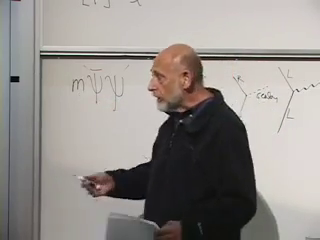
\includegraphics[width=0.76\textwidth]{lecture_01_figure_04.png}
\caption{費米子質量項，以及黑板上改變手徵性的線條示意圖。由於部分粉筆筆跡被遮住，以下會根據代數關係重建這些圖。}
\lectureframe{01:23:36}
\end{figure}

講課時常會說手性或螺旋度。若要精確描述這種保護機制，以手徵性表述最為清楚。對於超相對論性粒子，螺旋度的圖像可以提供直觀理解；不過，式~\eqref{eq:fermion-mass}中的左右手場所帶有的量是手徵性。

規範相互作用會保持手徵性：
\begin{equation}
L\xrightarrow{\ \gamma\ }L,
\qquad
R\xrightarrow{\ \gamma\ }R.
\label{eq:gauge-preserves-chirality}
\end{equation}
與標量場的湯川相互作用則會連結相反的手徵性：
\begin{equation}
L\xleftrightarrow{\ \phi\ }R.
\label{eq:scalar-flips-chirality}
\end{equation}
先假設電子以\(m_0=0\)開始。無論發射並重新吸收多少光子，都無法產生質量，因為每個規範頂點都保持手徵性。從左手開始的整個過程便會一直保持左手。因此，純量子電動力學可以一致地容許無質量電子：電磁自能無法在質量為零時產生額外的質量。

在線條圖像中，先從左手徵電子開始。經過第一個光子頂點後，它仍是左手徵；光子傳播並被重新吸收後，它依然是左手徵。重複這個過程只會加入更多保持手徵性的頂點。外部二點函數可以經過重整化，但不會因此產生定義質量所需的左右手結構。

發射標量粒子能做到嗎？一個標量頂點會將\(L\)轉變為\(R\)，但發射出的標量粒子必須再被吸收。因此，二點自能圖中會有偶數個標量頂點。第二次翻轉會抵銷第一次，所以完整的圖仍保持外部手徵性。無論內部圖有多複雜，發射與重新吸收都會使頂點成對出現，因而在起始質量為零時，無法產生可加的\(L\)到\(R\)項。

這是根據翻轉次數奇偶性所作的論證。一個標量頂點會使手徵性翻轉一次；每條內部標量線都必須閉合，因此需要另一個端點，也就需要第二次翻轉。四個標量頂點會造成四次翻轉，依此類推。翻轉偶數次後，費米子會回到原本的手徵性。這個結論不限於黑板上畫出的最簡單圈圖。

只有在圖中已經有質量插入時，才可能產生非零的質量修正。例如，光子的發射與重新吸收可以發生在一個\(m_0\bar\psi\psi\)插入的兩側。規範頂點帶來電荷的二次方，而唯一一次手徵性翻轉則帶入原有的質量：
\begin{equation}
\begin{aligned}
m_e
&=m_0+c_1e^2m_0+c_2e^4m_0+\cdots\\
&=m_0\left(1+c_1e^2+c_2e^4+\cdots\right).
\end{aligned}
\label{eq:multiplicative-fermion-mass}
\end{equation}
若\(m_0=0\)，結果仍為零。若\(m_0\)很小，每一項修正都正比於這個小量。我們仍可以追問，為什麼電子相對於基本尺度如此之輕；但不必再靠相減巨大而互不相關的數值來得到電子質量。就這個意義而言，小的費米子質量在技術上是自然的。

質量插入清楚展現了這個允許的過程。從\(L\)開始。光子發射會保持\(L\)；插入\(m_0\)後，\(L\)轉變為\(R\)；光子重新吸收則保持\(R\)。此時，圖的外部手徵性符合質量項的形式，但其數值必然含有因子\(m_0\)。這正是它與式~\eqref{eq:one-loop-scalar-mass}的關鍵差異：即使將起始標量質量設為零，式中的標量修正仍不為零。

規範玻色子也受到類似的保護：規範對稱性禁止獨立的質量項，因此起初無質量的規範玻色子，在所有微擾階數下都會保持無質量。在標準模型中，費米子和弱規範玻色子的質量來自對希格斯期望值的響應。只要控制好希格斯尺度，其餘輕粒子的質量就不必各自再經歷同樣災難性的微調。

這指出了超對稱意圖處理的問題：理論能否阻止希格斯標量獲得巨大的可加質量修正？在適當的超對稱架構中，答案是肯定的，因為玻色子與費米子的貢獻彼此相關，而非各自獨立。詳細機制將從下一講開始說明。

\section{另一種微調：真空能量}

還有一個更嚴重的重整化問題，但只有納入引力後才會成為可觀測現象。在非引力物理中，對所有能量加上同一個常數，不會改變任何實驗結果。例如，電子質量不是絕對能量，而是從真空中加入一個電子所需的額外能量：
\begin{equation}
m_e=E(\text{vacuum}+\text{one electron})-E(\text{vacuum})
\end{equation}
這是在電子靜止系中定義的。若真空與所有激發態的能量一起平移，它們之間的差值便保持不變。

然而，真空到真空的圖確實會改變真空能量。在\(\lambda\phi^4\)理論中，將一個四次頂點的四條線接成兩個短迴圈。每個重合的傳播子都貢獻\(1/\delta^2\)，因此
\begin{equation}
\delta\rho_{\mathrm{vac}}
\sim
c_{\mathrm{vac}}\frac{\lambda}{\delta^4}.
\label{eq:vacuum-energy-divergence}
\end{equation}
更複雜的真空圖會帶有不同的耦合因子和係數，但量綱分析通常仍會得到相同的四次截斷尺度依賴，出現在能量密度中。

沒有外部線，正是辨認這項修正的關鍵。二點圖比較單粒子態與真空，因而改變質量；四點圖會改變散射；沒有入射或出射粒子的圖，則會改變真空到真空的振幅本身。一個四次頂點帶來\(\lambda\)，它的兩個短迴圈則各帶來\(\delta^{-2}\)。依量綱分析，能量密度便會具有\(\delta^{-4}\)的尺度。

沒有引力時，人們可以任意選定能量的零點，並且認為這不會造成影響。廣義相對論則取消了這項自由：應力能量會產生時空曲率，因此均勻的真空能量也會使空無一物的空間產生引力。真空能量表現為宇宙常數，並在觀測上與暗能量相關。因此，實測到的微小真空能量必須在形如\(\delta^{-4}\)的貢獻之下仍保持微小。

這就是納入引力後，問題為何會改變。在普通量子力學中，將每個能階都平移同一個常數，不會改變躍遷頻率。在引力中，這個常數並非無關緊要：真空的應力張量正比於度規，會使時空彎曲。原本任意選定的能量零點，於是成了愛因斯坦方程中的源。

因此，至少存在兩個極端的自然性難題。講座估計，真空能量的微調約涉及123位小數，希格斯質量的微調則約涉及30--35位。確切數目取決於紫外尺度與採用的慣例，但兩者差異之大毫無疑問。超對稱或許能回應這裡討論的希格斯問題；然而，超對稱一旦破缺，本身並不能解釋觀測到的宇宙常數。\editorialnote{這也說明了為什麼精確超對稱下玻色子--費米子的相消，無法在現象學上解決觀測到的真空能量問題：我們的世界中超對稱必須破缺。}

\section{課堂提問總結}

\begin{classroomqa}
\audiencequestion{希格斯修正取決於截斷尺度\(\delta\)，但截斷尺度似乎是任意的。它可以是普朗克長度、普朗克長度的十倍，或是別的尺度嗎？這是否代表微調也是任意的？\lecturetimestamp{01:33:50}}
\lecturerresponse{數值貢獻取決於有效理論所適用的最短尺度。這種依賴是物理計算的一部分，不能藉此迴避問題。只要標準模型在某個尺度上仍然適用，該尺度的模式及其效應就必須納入計算。可以選擇在預期新物理出現的距離處設定\(\delta\)---，例如普朗克尺度，或接近\(10^{16}\,\mathrm{GeV}\)的大統一尺度。累積到該尺度的貢獻，已經構成這個問題的一個下限。若將同一理論延伸至更短距離，二次敏感性只會更大。我們必須解釋，從實驗室尺度到那個紫外邊界之間，各個尺度的貢獻是如何被抵消的。}
\end{classroomqa}

\begin{classroomqa}
\audiencequestion{如何定義標量粒子？有什麼例子？\lecturetimestamp{01:37:26}}
\lecturerresponse{希格斯粒子就是這裡要舉的例子。標量在空間旋轉下不會轉變成不同的分量；換言之，它的粒子量子自旋為零。光子以向量場描述，引力場則以張量描述。在2010這場講座進行時，還沒有探測到任何基本的零自旋粒子。\editorialnote{希格斯玻色子於2012年在 CERN 被發現，其測量性質與零自旋相符。}}
\end{classroomqa}

\begin{classroomqa}
\audiencequestion{\(Z\)粒子也是規範玻色子嗎？\lecturetimestamp{01:38:31}}
\lecturerresponse{是。\(Z\)、\(W^+\)和\(W^-\)都是自旋為 1 的規範玻色子，光子也是如此。它們的場方程與相互作用，是麥克斯威式規範描述在非阿貝爾或電弱理論中的推廣。}
\end{classroomqa}

\begin{classroomqa}
\audiencequestion{為什麼玻色子的基態貢獻不會抵消真空能量中的費米子貢獻？\lecturetimestamp{01:39:10}}
\lecturerresponse{費米子迴圈與相應的玻色子迴圈，確實可能以相反符號出現。但抵消並非自動發生：粒子的質量、多重度和耦合都必須匹配。即使只有些微差異，也會留下對截斷尺度敏感的巨大殘值；而無窮多族的圖也必須逐階匹配。精確超對稱會強制玻色子--費米子之間存在這類關係。一般的非超對稱粒子內容則不會如此；超對稱破缺後，真空能量問題仍會留下。}
\end{classroomqa}

\section{展望}

本講的安排有其用意。首先，分子計算說明消去快變數既不是忽略它們，也不是變魔術：快變數的基態能量會成為慢變數的勢能。量子場論則在不同波長上重複這項操作。接著，量綱分析揭示哪些有效參數會對截斷尺度敏感。標量質量會得到正比於\(\delta^{-2}\)的加性項，因此小的希格斯尺度顯得異常脆弱。手徵性保護零質量極限，使費米子質量接受乘性重整化；規範對稱性也同樣保護無質量規範玻色子。真空能量的敏感性更高，按\(\delta^{-4}\)的尺度變化；引力則使它的絕對值成為可觀測量。

超對稱正是在這個時刻進入課程：它不是裝飾性的新數學，而是試圖讓標量部門的表現更接近受到保護的部門。接下來要理解的是，什麼樣的對稱性可以將玻色子和費米子緊密聯繫起來，並藉此組織這些相消。